\documentclass{article}
\usepackage[utf8]{inputenc}
\usepackage[portuges]{babel}
\usepackage{csquotes}
\usepackage{geometry}
\usepackage[pdftex]{hyperref}
\usepackage{indentfirst}
\usepackage{amsthm}
\usepackage{amssymb}
\usepackage{amsmath}
\usepackage{mathrsfs}
\usepackage{graphicx}
\usepackage{float}
\usepackage{multicol}
\usepackage{verbatim}

\newtheorem{definition}{Definição}
\newtheorem{theorem}{Teorema}
\newtheorem{lemma}[theorem]{Lema}
\newtheorem{example}{Exemplo}

\usepackage[backend = biber]{biblatex}
\addbibresource{terceiro_trabalho.bib}

\geometry{left = 3cm, top = 3cm, bottom = 2cm, right = 2cm}

\title{Inferência Estatística \\ 3º Trabalho}
\author{Igor Patrício Michels}
\date{21/10/2020}

\begin{document}

\maketitle

\section*{Introdução}

Trabalho elaborado pelo aluno Igor Patrício Michels referente a disciplina de Inferência Estatística, do quarto período da Graduação em Matemática Aplicada da FGV-EMAp. Nele faremos uma análise bayesiana da distribuição normal.

O enunciado e eventuais funções utilizadas para resolução deste ou de outros trabalhos podem ser encontrados \href{https://github.com/IgorMichels/Statistical_Inference}{\textbf{nesse repositório do GitHub}}.

\section*{Uma Análise Bayesiana no Caso Normal}

\subsection*{Precisão}

Antes de começar nossa análise vamos definir o termo precisão, bem como dar uma pequena intuição de seu significado.

\begin{definition}
    Seja $\sigma^2$ a variância de uma distribuição. O parâmetro $\tau = \left(\sigma^2\right)^{-1}$ é chamado de precisão.
\end{definition}

Note que a precisão é definida como o recíproco da variância, uma medida de dispersão dos dados. Assim, se possuímos uma variância baixa afirmar ver que os valores tenderam a estarem próximos da média da distribuição. Já se a variância é alta os valores poderão estar mais espalhados ao redor da média, como ilustrado na figura \ref{gaussianas}.
\begin{figure}[H]
    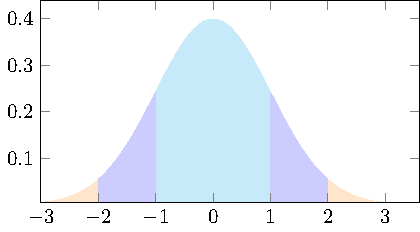
\includegraphics[page = 1]{3º Trabalho/Tikz - pdf/Tikz1.pdf}
    \includegraphics[page = 2]{3º Trabalho/Tikz - pdf/Tikz1.pdf}
    \caption{à esquerda temos a plotagem de uma $\mathcal{N}(0, 1^2)$, já à direita a plotagem de uma $\mathcal{N}(0, 2^2)$.}
    \label{gaussianas}
\end{figure}

Note que na figura \ref{gaussianas} ambas as p.d.f.'s são iguais, com exceção a escala, a qual foi modificada em virtude da mudança na variância. Esse detalhe nos possibilita perceber a regra 68-95-99.7\footnote{A regra 68-95-99.7 é a propriedade de que aproximadamente 68\% dos valores estão a menos de um desvio padrão da média da normal, bem como 95\% e 99.7\% estão a uma distância inferior a dois e três desvios padrão, respectivamente.} da normal, além de reforçar a ideia de que, quanto maior a variância, maior a dispersão dos valores em torno da média.\footnote{Aqui poderíamos apenas citar a regra 96-95-99.7, entretanto a plotagem da distribuição da normal facilita o entendimento, uma vez que a forma da curva permanece a mesma, mas a escala do eixo $x$ aumenta.}

Dessa forma, a precisão pode ser considerada uma medida de proximidade dos dados, pois a precisão é definida como o recíproco da variância. Assim, quando temos uma variância baixa os valores se encontram perto da média e a precisão é alta, já quando a variância é grande os valores estão mais dispersos e a precisão é menor.

Definida a ideia de precisão podemos nos perguntar qual a utilidade da mesma além de ser uma métrica como citado anteriormente. Podemos responder a essa dúvida mostrando qual a função de densidade de probabilidade de uma variável com distribuição normal em cada uma das parametrizações:
\[X \sim \mathcal{N}(\mu, \sigma^2) \longrightarrow f_X(x \mid \mu, \tau) = \dfrac{1}{\sqrt{2\pi \sigma^2}}\exp{\left[-\dfrac{1}{2}\left(\dfrac{x - \mu}{\sigma}\right)^2\right]}\]
\[X \sim \mathcal{N}_2(\mu, \tau) \longrightarrow f_X(x \mid \mu, \tau) = \sqrt{\dfrac{\tau}{2\pi}}\exp{\left[-\dfrac{1}{2}\tau(x - \mu)^2\right]},\]

\noindent onde $\mathcal{N}_2$ representa a normal parametrizada com a média e precisão. Já para uma distribuição conjunta temos as seguintes parametrizações:
\begin{itemize}
    \item
        se $X_1, \dots, X_n \sim \mathcal{N}(\mu, \sigma^2)$:
        \begin{equation*}
            \begin{split}
                f_X(x_1, \dots, x_n \mid \mu, \tau) & = \prod_{i = 1}^{n} \dfrac{1}{\sqrt{2\pi \sigma^2}}\exp{\left[-\dfrac{1}{2}\left(\dfrac{x_i - \mu}{\sigma}\right)^2\right]} \\
                & = \left(\dfrac{1}{\sqrt{2\pi \sigma^2}}\right)^n \prod_{i = 1}^{n} \exp{\left[-\dfrac{1}{2}\left(\dfrac{x_i - \mu}{\sigma}\right)^2\right]} \\
                & = \left(\sqrt{2\pi \sigma^2}\right)^{-\frac{n}{2}} \exp{\left[-\dfrac{1}{2\sigma^2}\sum_{i = 1}^{n}\left(x_i - \mu\right)^2\right]} \\
            \end{split}
        \end{equation*}
        
    \item
        já se $X_1, \dots, X_n \sim \mathcal{N}_2(\mu, \tau)$:
        \begin{equation}
            \label{eq1}
            \begin{split}
                f_X(x_1, \dots, x_n \mid \mu, \tau) & = \prod_{i = 1}^{n} \sqrt{\dfrac{\tau}{2\pi}}\exp{\left[-\dfrac{1}{2}\tau(x_i - \mu)^2\right]} \\
                & = \left(\sqrt{\dfrac{\tau}{2\pi}}\right)^n \prod_{i = 1}^{n} \exp{\left[-\dfrac{1}{2}\tau\left(x_i - \mu\right)^2\right]} \\
                & = \left(\sqrt{\dfrac{\tau}{2\pi}}\right)^n \exp{\left[-\dfrac{1}{2}\tau\sum_{i = 1}^{n}\left(x_i - \mu\right)^2\right]} \\
            \end{split}
        \end{equation}
\end{itemize}

Perceba que, nos dois casos, a segunda representação é mais amigável, uma vez que é mais fácil de manipular os parâmetros manualmente pois não ocorrem divisões por um parâmetro, o que pode ser complicado. Além disso, com essa segunda representação podemos perceber facilmente pequenas variações \cite{stackexchange}.

\subsection*{Inferência utilizando a Precisão}

Dada a distribuição conjunta condicional dos dados em \ref{eq1}, podemos buscar uma distribuição a priori para $\mu$ e $\tau$. Assim como em \cite{ehlers} e \cite{ehlers2}, vamos reescrever $P(\mu, \tau) = P(\mu \mid \tau)\cdot P(\tau)$, dessa forma, vamos encontrar uma priori em duas etapas. Na primeira etapa, note que, dado $\tau$, a distribuição conjunta tem a forma de uma normal, assim escrevemos
\[\mu \mid \tau \sim \mathcal{N}_2(\mu_0, \lambda_0 \tau).\]

Já para a segunda etapa, quando precisamos encontrar a priori de $\tau$, podemos notar que, do ponto de vista de $\tau$, o núcleo da distribuição em \ref{eq1} tem a mesma forma que o núcleo de uma distribuição Gama. Dessa forma, temos que
\[\tau \sim \text{Gama}\left(\alpha_0, \beta_0\right).\]

Já para o cálculo da posteriori, podemos seguir uma ideia similar a que DeGroot fez em \cite{degroot}. Sejam $\xi_1$ e $\xi_2$ as prioris de $\mu \mid \tau$ e $\tau$, respectivamente. Assim, temos que
\[\xi_1(\mu \mid \tau) \propto \sqrt{\tau} \exp{\left[-\dfrac{1}{2}\lambda_0 \tau (\mu - \mu_0)^2\right]} \text{ e que } \xi_2(\tau) \propto \tau^{\alpha_0 - 1} \exp{\left[- \beta_0 \tau\right]}.\]

Dessa forma, a posteriori da distribuição conjunta deve satisfazer
\begin{equation}
    \label{post1}
    \begin{split}
        \xi(\mu, \tau \mid x_1, x_2, \dots, x_n) & \propto f_X(x_1, \dots, x_n \mid \mu, \tau) \xi_1(\mu \mid \tau) \xi_2(\tau) \\
        & \propto \tau^{\alpha_0 - 1 + (n + 1)/2} \exp{\left[-\dfrac{\tau}{2}\left(\lambda_0 (\mu - \mu_0)^2 + \sum_{i = 1}^{n}\left(x_i - \mu\right)^2\right) - \beta_0 \tau\right]}.
    \end{split}
\end{equation}

Agora, perceba que
\begin{equation*}
    \begin{split}
        \sum_{i = 1}^{n} \left(x_i - \mu\right)^2 & = \sum_{i = 1}^{n} \left(x_i - \overline{x}_n + \overline{x}_n - \mu\right)^2 \\
        & = \sum_{i = 1}^{n} \left[\left(x_i - \overline{x}_n\right)^2 + 2\left(x_i - \overline{x}_n\right)\left(\overline{x}_n - \mu\right) + \left(\overline{x}_n - \mu\right)^2\right] \\
        & = \sum_{i = 1}^{n} \left(x_i - \overline{x}_n\right)^2 + \sum_{i = 1}^{n} 2\left(x_i - \overline{x}_n\right)\left(\overline{x}_n - \mu\right) + \sum_{i = 1}^{n} \left(\overline{x}_n - \mu\right)^2 \\
        & = \overline{s}_n^2 + 2\left(\overline{x}_n - \mu\right)\sum_{i = 1}^{n} \left(x_i - \overline{x}_n\right) + n\left(\overline{x}_n - \mu\right)^2 \\
        & = \overline{s}_n^2 + 2\left(\overline{x}_n - \mu\right)\cdot 0 + n\left(\overline{x}_n - \mu\right)^2 \\
        & = \overline{s}_n^2 + n\left(\overline{x}_n - \mu\right)^2.
    \end{split}
\end{equation*}

Assim, podemos reescrever \ref{post1} como
\begin{equation}
    \label{post2}
    \xi(\mu, \tau \mid x_1, x_2, \dots, x_n) \propto \tau^{\alpha_0 - 1 + (n + 1)/2} \exp{\left[-\dfrac{\tau}{2}\left(\lambda_0 (\mu - \mu_0)^2 + \overline{s}_n^2 + n\left(\overline{x}_n - \mu\right)^2\right) - \beta_0 \tau\right]}.
\end{equation}

Note também que
\begin{equation}
    \label{ig}
    \begin{split}
        n\left(\overline{x}_n - \mu\right)^2 + \lambda_0\left(\mu - \mu_0\right)^2 & = n\overline{x}_n^2 - 2n\overline{x}_n\mu + n\mu^2 + \lambda_0\mu^2 - 2\lambda_0\mu\mu_0 + \lambda_0\mu_0^2 \\
        & = (n + \lambda_0)\left(\mu^2 - \dfrac{2n\overline{x}_n\mu + 2\lambda_0\mu\mu_0}{n + \lambda_0} + \dfrac{\left(n + \lambda_0\right)\left(n\overline{x}_n^2 + \lambda_0\mu_0^2\right)}{\left(n + \lambda_0\right)^2}\right),
    \end{split}
\end{equation}

\noindent desenvolvendo a última fração de \ref{ig} separadamente, temos
\begin{equation*}
    \begin{split}
        \dfrac{\left(n + \lambda_0\right)\left(n\overline{x}_n^2 + \lambda_0\mu_0^2\right)}{\left(n + \lambda_0\right)^2} & = \dfrac{n^2\overline{x}_n^2 + n\lambda_0\mu_0^2 + n\lambda_0\overline{x}_n^2 + \lambda_0^2\mu_0^2}{\left(n + \lambda_0\right)^2} \\
        & = \dfrac{\lambda_0^2\mu_0^2 + 2\mu_0\lambda_0n\overline{x}_n + n^2\overline{x}_n^2 + n\lambda_0\overline{x}_n^2 - 2\mu_0\lambda_0n\overline{x}_n + n\lambda_0\mu_0^2}{\left(n + \lambda_0\right)^2} \\
        & = \dfrac{\left(\lambda_0^2\mu_0^2 + 2\mu_0\lambda_0n\overline{x}_n + n^2\overline{x}_n^2\right) + n\lambda_0 \left(\overline{x}_n^2 - 2\mu_0\overline{x}_n + \mu_0^2\right)}{\left(n + \lambda_0\right)^2} \\
        & = \dfrac{\left(\lambda_0\mu_0 + n\overline{x}_n\right)^2 + n\lambda_0 \left(\overline{x}_n - \mu_0\right)^2}{\left(n + \lambda_0\right)^2}.
    \end{split}
\end{equation*}

Substituindo isso em \ref{ig}, temos
\begin{equation*}
    \begin{split}
        n\left(\overline{x}_n - \mu\right)^2 + \lambda_0\left(\mu - \mu_0\right)^2 & = (n + \lambda_0)\left(\mu^2 - \dfrac{2n\overline{x}_n\mu + 2\lambda_0\mu\mu_0}{n + \lambda_0} + \dfrac{\left(\lambda_0\mu_0 + n\overline{x}_n\right)^2 +  n\lambda_0 \left(\overline{x}_n - \mu_0\right)^2}{\left(n + \lambda_0\right)^2}\right) \\
        & = (n + \lambda_0)\left(\mu^2 - \dfrac{2\mu \left(n\overline{x}_n + \lambda_0\mu_0\right)}{n + \lambda_0} + \dfrac{\left(\lambda_0\mu_0 + n\overline{x}_n\right)^2}{\left(n + \lambda_0\right)^2}\right) + \dfrac{n\lambda_0 \left(\overline{x}_n - \mu_0\right)^2}{n + \lambda_0} \\
        & = (n + \lambda_0)\left(\mu - \dfrac{\lambda_0\mu_0 + n\overline{x}_n}{n + \lambda_0}\right)^2 + \dfrac{n\lambda_0 \left(\overline{x}_n - \mu_0\right)^2}{n + \lambda_0}.
    \end{split}
\end{equation*}

Dessa forma, substituindo o resultado acima em \ref{post2}, obtemos
\begin{equation*}
    \xi(\mu, \tau \mid x_1, x_2, \dots, x_n) \propto \tau^{\alpha_0 - 1 + (n + 1)/2} \exp{\left[-\dfrac{\tau}{2}\left(\overline{s}_n^2 + (n + \lambda_0)\left(\mu - \dfrac{\lambda_0\mu_0 + n\overline{x}_n}{n + \lambda_0}\right)^2 + \dfrac{n\lambda_0 \left(\overline{x}_n - \mu_0\right)^2}{n + \lambda_0}\right) - \beta_0 \tau\right]}.
\end{equation*}

Definindo
\begin{equation*}
    \begin{split}
        \lambda_1 & = \lambda_0 + n \\
        \mu_1 & = \dfrac{\lambda_0\mu_0 + n\overline{x}_n}{n + \lambda_0} \\
        \alpha_1 & = \alpha_0 + \dfrac{n}{2} \\
        \beta_1 & = \beta_0 + \dfrac{\overline{s}_n^2}{2} + \dfrac{n\lambda_0\left(\overline{x}_n - \mu_0\right)^2}{2\left(\lambda_0 + n\right)},
    \end{split}
\end{equation*}

\noindent podemos escrever o termo dentro da exponencial como\footnote{Como as expressões são muito grandes, estou manipulando as mesmas de uma linha para outra.}
\[-\dfrac{\tau}{2}\left(\overline{s}_n^2 + (n + \lambda_0)\left(\mu - \dfrac{\lambda_0\mu_0 + n\overline{x}_n}{n + \lambda_0}\right)^2 + \dfrac{n\lambda_0 \left(\overline{x}_n - \mu_0\right)^2}{n + \lambda_0}\right) - \beta_0 \tau\]
\[-\dfrac{1}{2}\left(\lambda_0 + n\right)\tau\left(\mu - \left(\dfrac{\lambda_0\mu_0 + n\overline{x}_n}{n + \lambda_0}\right)\right)^2 - \tau\left(\beta_0 + \dfrac{\overline{s}_n^2}{2} + \dfrac{n\lambda_0 \left(\overline{x}_n - \mu_0\right)^2}{2\left(n + \lambda_0\right)}\right)\]
\[-\dfrac{1}{2}\lambda_1\tau\left(\mu - \mu_1\right)^2 - \tau\beta_1.\]

Já o expoente de $\tau$ pode ser escrito como
\begin{equation*}
    \begin{split}
        \alpha_0 - 1 + \dfrac{n + 1}{2} & = \alpha_0 + \dfrac{n}{2} - 1 + \dfrac{1}{2} \\
        & = \alpha_1 - 1 + \dfrac{1}{2}.
    \end{split}
\end{equation*}

Dessa forma, temos

\begin{equation*}
    \begin{split}
        \xi(\mu, \tau \mid x_1, x_2, \dots, x_n) & \propto \tau^{\alpha_1 - 1 + 1/2} \exp{\left[-\dfrac{1}{2}\lambda_1\tau\left(\mu - \mu_1\right)^2 -\beta_1\tau\right]} \\
        & = \tau^{1/2} \exp{\left[-\dfrac{1}{2}\lambda_1\tau\left(\mu - \mu_1\right)^2\right]} \cdot \tau^{\alpha_1 - 1} \exp{\left[-\beta_1\tau\right]}.
    \end{split}
\end{equation*}

Assim, obtemos a distribuição conjunta a posteriori de $\mu$ e $\tau$. Além disso, o termo
\[\tau^{1/2} \exp{\left[-\dfrac{1}{2}\lambda_1\tau\left(\mu - \mu_1\right)^2\right]},\]

\noindent é, exceto por um fator que independe de $\mu$ e $\tau$, a distribuição a posteriori de $\mu \mid \tau$, sendo da forma Normal$_2$ com média $\mu_1$ e precisão $\lambda_1\tau$. Já o termo
\[\tau^{\alpha_1 - 1} \exp{\left[-\beta_1\tau\right]}\]

\noindent é, também exceto por um fator multiplicativo que independe de $\mu$ e $\tau$, a distribuição a posteriori de $\tau$. Note que essa distribuição é uma Gama de parâmetros $\alpha_1$ e $\beta_1$.

Esse conjunto de prioris utilizadas acima para esse caso normal em que desconhecemos tanto a média quanto a precisão é conhecida como Distribuição Normal-Gama. Note que essa distribuição é fechada no cálculo da posteriori, ou seja, a posteriori tem a mesma distribuição da priori. Já a distribuição marginal de $\mu$ a posteriori pode ser encontrada integrando o produto de $P(\tau)$ com $P(\mu \mid \tau)$ no domínio de $\tau$, isto é $\mathbb{R}_{>0}$. Fazendo isto, temos
\begin{equation*}
    \begin{split}
        P(\mu) & = \int_{0}^{\infty} P(\mu \mid \tau) P(\tau) ~d\tau \\
        & \propto \int_{0}^{\infty} \tau^{1/2} \exp{\left[-\dfrac{1}{2}\lambda_1\tau\left(\mu - \mu_1\right)^2\right]} \tau^{\alpha_1 - 1} \exp{\left[-\beta_1\tau\right]} ~d\tau \\
        & \propto \int_{0}^{\infty} \tau^{\alpha_1 - 1 + 1/2} \exp{\left[-\dfrac{1}{2}\lambda_1\tau\left(\mu - \mu_1\right)^2 - \beta_1\tau\right]} ~d\tau \\
        & \propto \left(\dfrac{2\beta_1 + \lambda_1 \left(\mu - \mu_1\right)^2}{2}\right)^{-\left(\alpha_1 + \frac{1}{2}\right)} \\
        & \propto \left(1 + \dfrac{\left(\mu - \mu_1\right)^2}{\frac{2\beta_1}{\lambda_1}}\right)^{-\left(\alpha_1 + \frac{1}{2}\right)},
    \end{split}
\end{equation*}

\noindent onde podemos ver que $\mu$ tem distribuição $t$ deslocada, isto é,
\[\mu \sim X = \mu_1 + \left(\dfrac{\beta_1}{\alpha_1 \lambda_1}\right)^{\frac{1}{2}}T,\]

\noindent com $T$ tendo distribuição $t$ de Student com $2\alpha_1$ graus de liberdade.

\subsubsection*{Paralelo com o Frequentismo}

Fazendo um paralelo com a ideia frequentista, note que a média a posteriori $\left(\mu_1\right)$ é função da média amostral $\left(\overline{x}_n\right)$, que é o EMV, e dos hiperparâmetros iniciais:
\[\mu_1 = \dfrac{\lambda_0\mu_0 + n\overline{x}_n}{n + \lambda_0}.\]

Note que o lado direito da expressão acima pode ser interpretada como uma média ponderada entre $\mu_0$ e $\overline{x}_n$. Dessa forma, $\mu_0$ tem peso $\lambda_0$ e $\overline{x}_n$ tem peso $n$ e, com isso, nota-se que quando o número de amostras cresce $(n \to \infty)$, temos que $\mu_1 \to \overline{x}_n$. Dessa forma, podemos interpretar $\lambda_0$ como se fosse uma espécie de ``métrica de certeza'' ou então uma ``métrica de aversão'' em relação as ideias, a priori, sobre $\mu_0$, como se você tivesse feito o experimento anteriormente $\lambda_0$ vezes, obtendo uma média $\mu_0$.

Exemplificando essa ideia, tomando $\mu_0$ e $\lambda_0 > n$ teremos, após a atualização dos hiperparâmetros, um valor de $\mu_1$ mais próximo de $\mu_0$ que de $\overline{x}_n$. Dessa forma, um $\lambda_0$ maior que $n$ implica que, de certo modo, estamos confiando mais nos conhecimentos prévios sobre o experimento que em nossas observações. Podemos notar também que, se $\lambda_0 \gg n$, a diferença entre $\mu_1$ e $\mu_0$ é muito pequena, o que pode nos levar a ideia do parágrafo anterior, ou seja, a de considerar $\lambda_0$ como uma ``métrica de certeza'' ou uma ``métrica de aversão'', assim, quanto maior $\lambda_0$, podemos dizer que estamos mais certos que sobre $\mu$ a partir de nossa ideia $\mu_0$ ou então que estamos mais aversos a alterações na atualização do parâmetro $\mu_0$. Note que, nos dois casos, necessitamos uma grande quantidade de amostras para uma alteração significativa de $\mu_0$ para $\mu_1$, quando a mesma for possível.\footnote{Note que podemos ter $\mu_0$ muito próximo do valor esperado de $\mu$, então ter um $\lambda_0$ alto, indicando certeza ou aversão, acaba não sendo relevante, pois o esperado é que, com $n$ grande, $\overline{x}_n$ também esteja próximo ao valor esperado de $\mu$, logo, as diferença entre $\mu_0$ e $\mu_1$ acaba se tornando pequena, mesmo com $\lambda_0$ pequeno.} Uma outra visualização para $\lambda_0$ seria como quantidade de pseudo-observações, como se você já tivesse realizado esse experimento em algum momento anteriormente, obtendo média $\mu_0$.

Já os hiperparâmetros $\alpha_i$ e $\beta_i$ acabam, conforme resultado acima, dando forma a distribuição de $\mu$. Além disso, note que $\alpha_0$ e $\beta_0$ são proporcionais, assim, podemos escolher $\alpha_0$ e, feito isso, temos $\beta_0$. Dessa forma, podemos interpretar $\alpha_0$ como se fosse a quantidade de pseudo-observações já realizadas.

Após termos visto o desenvolvimento das distribuições a posteriori vamos ilustrar essas ideias com um exemplo.

\subsection*{Um pequeno exemplo}

\begin{example}
    Palmirinha anda preocupada com a concentração de amido em sua pamonha. Ela pede para Valciclei, seu assistente, amostrar $n=10$ pamonhas e medir sua concentração de amido.
    
    Ele, muito prestativo, rapidamente faz o experimento, mas, porque comeu todas as amostras depois que foram medidas, precisou fazer uma visita de emergência ao banheiro. Desta feita, apenas teve tempo de anotar em um papel a média e variância amostrais, $\bar{x}_n =  8.307849$ e $\bar{s}^2_n = 7.930452$.
    
    Palmirinha tem uma reunião com investidores em pouco tempo, então decide voltar aos seus tempos de bayesiana~\textit{old school} e analisar os dados utilizando prioris conjugadas. Ela supõe que a concentração de amido segue uma distribuição normal com parâmetros $\mu$ e $\tau$ e que as observações feitas por Valciclei são independentes entre si. Ela suspeita que a concentração de amido na pamonha fique em torno de $10$ mg/L, com desvio padrão de $2$ mg/L. Com sua larga experiência na confecção de pamonhas, ela suspeita ainda que o coeficiente de variação da concentração de amido seja em torno de $1/2$. Palmirinha tem um quadro em seu escritório, que diz
    \[\operatorname{cv} = \frac{\sigma}{\mu}.\]
    
    Agora, 
    \begin{enumerate}
        \item
            Com os dados anotados por Valciclei, é possível computar a distribuição~\textit{a posteriori} de $\mu$ e $\tau$? Justifique.
            
        \item
            Em caso afirmativo, ajude Palmirinha a encontrar $a, b \in \mathbb{R}$, $a < b$ de modo que $\operatorname{Pr}(\mu \in (a, b) \mid \boldsymbol{x}) = 0.95$.
    \end{enumerate}
\end{example}

Nesse exemplo, apesar de parecer que não é possível encontrar a distribuição a posteriori de $\mu$ e $\tau$, é possível sim, conforme visto anteriormente, encontrar tal distribuição. Abaixo temos duas soluções.

\subsubsection*{Uma solução}

Primeiramente, note que, dados $\lambda_0$, $\mu_0$, $\alpha_0$ e $\beta_0$, necessitamos apenas de $n$, $\overline{x}_n$ e $\overline{s}_n^2$ para computar os parâmetros da distribuição a posteriori, a qual já vimos ser Normal-Gama. Agora, perceba que Valciclei fez suas estatística baseado em dados de dez pamonhas, ou seja, $n = 10$. Além disso, as estatísticas que Valciclei conseguiu anotar antes de fazer sua visita de emergência ao banheiro foram, justamente, a média amostral $\left(\overline{x}_n\right)$ e a variância amostral $\left(\overline{s}_n^2\right)$.

Agora precisamos apenas verificar quais são os hiperparâmetros para nossa priori. Note que Palmirinha suspeita que a concentração de amido está em torno de $10$ mg/L, ou seja, tomamos $\mu_0 = 10$.

Agora, sabemos que Palmirinha suspeita que o desvio padrão da concentração seja igual a $2$, ou seja, uma variância igual a $4$, além de sua suspeita de que o coeficiente de variação esteja próximo de $\frac{1}{2}$. Equacionando essas informações, já usando que $\mu_0 = 10$, temos:
\[\sigma^2 = 4 \implies \tau = \dfrac{1}{4} \implies \dfrac{\beta_0}{\alpha_0} = \dfrac{1}{4} \text{ e } \operatorname{cv} = \dfrac{\sigma}{\mu} = \dfrac{\sqrt{\tau^{-1}}}{\mu} \implies E\left[\operatorname{cv} \mid \mu_0 = 10\right] = \dfrac{\sqrt{\alpha_0}}{10\cdot \sqrt{\beta_0}} \implies \dfrac{1}{2} = \dfrac{\sqrt{\alpha_0}}{10\cdot \sqrt{\beta_0}}.\]

Note que os dois resultados acima são excludentes, uma vez que devemos ter
\[\dfrac{1}{4} = \dfrac{\beta_0}{\alpha_0} = \dfrac{1}{25}.\]

Sendo assim, irei encontrar o parâmetro com $4$ prioris distintas:
\begin{itemize}
    \item
        usando que $\frac{\beta_0}{\alpha_0} = \frac{1}{4}$;
        
    \item
        usando que $\frac{\beta_0}{\alpha_0} = \frac{1}{25}$;
        
    \item
        usando que $\frac{\beta_0}{\alpha_0}$ é média aritmética entre $\frac{1}{4}$ e $\frac{1}{25}$, ou seja, $\frac{29}{200}$ e;
        
    \item
        usando que $\frac{\beta_0}{\alpha_0}$ é média geométrica entre $\frac{1}{4}$ e $\frac{1}{25}$, ou seja, $\frac{1}{10}$.
\end{itemize}

Note que, dessa forma, escolhendo $\alpha_0$, já temos o valor de $\beta_0$. Agora, precisamos encontrar o valor de $\lambda_0$. Para tanto, podemos utilizar o teorema 8.6.3 do DeGroot \cite{degroot}, o qual afirma que, com $\alpha_0 > 1$,
\[Var(\mu) = \dfrac{\beta_0}{\lambda_0 \left(\alpha_0 - 1\right)} \implies \lambda_0 = \dfrac{\beta_0}{Var(\mu) \left(\alpha_0 - 1\right)}.\]

Note que agora nosso problema passa a ser determinar um valor para $Var(\mu)$, o que podemos fazer de forma similar ao que DeGroot fez em seu exemplo 8.6.3, dividindo a variância amostral entre $Var(\mu)$ e $E[\tau]$. Fazendo
\[Var(\mu) = \dfrac{\overline{s}_n^2}{2} = 3.965226 \text{ e } E[\tau] = \dfrac{1}{\frac{\overline{s}_n^2}{2}} = \dfrac{1}{3.965226},\]

\noindent já temos o valor de $Var(\mu)$ e, consequentemente, podemos encontrar $\lambda_0$ ao tomar um $\alpha_0 > 1$ e, além disso, obtemos que o valor esperado de $\tau$ está próximo a $\frac{1}{4}$, que é o que Palmirinha estava supondo. Dessa forma, podemos fazer as contas nos quatro casos dados acima. Para isso, necessitamos escolher um valor para $\alpha_0$, assim, optarei por sempre escolher o valor que se encontra no denominador da fração que representa $\frac{\beta_0}{\alpha_0}$. Consequentemente, $\beta_0$ sempre o numerador da fração. Os cálculos de $\lambda_0$, bem como dos hiperparâmetros a posteriori e do intervalo de credibilidade foram realizados em um Notebook com Python 3.

Assim, no primeiro caso, onde $\frac{\beta_0}{\alpha_0} = \frac{1}{4}$, temos:
\begin{equation*}
    \left\{
        \begin{array}{ll}
            \alpha_0 & = 4 \\
            \beta_0 & = 1 \\
            \mu_0 & = 10 \\
            Var(\mu) & = 3.965226 \\
            n & = 10 \\
            \overline{x}_n & = 8.307849 \\
            \overline{s}_n^2 & = 7.930452
        \end{array}
    \right.
    \implies \lambda_0 \approx 0.08406414497769694,
\end{equation*}

\noindent o que nos retorna os seguintes hiperparâmetros a posteriori:
\begin{equation*}
    \left\{
        \begin{array}{ll}
            \lambda_1 & = 10.084064144977697 \\
            \mu_1 & = 8.321955338966417 \\
            \alpha_1 & = 9 \\
            \beta_1 & = 5.084576277941813
        \end{array}
    \right.
\end{equation*}

\noindent e o intervalo de credibilidade $(7.824678461062495, 8.819232216870338)$.

Já no segundo caso, quando $\frac{\beta_0}{\alpha_0} = \frac{1}{25}$, temos:
\begin{equation*}
    \left\{
        \begin{array}{ll}
            \alpha_0 & = 25 \\
            \beta_0 & = 1 \\
            \mu_0 & = 10 \\
            Var(\mu) & = 3.965226 \\
            n & = 10 \\
            \overline{x}_n & = 8.307849 \\
            \overline{s}_n^2 & = 7.930452
        \end{array}
    \right.
    \implies \lambda_0 \approx 0.010508018122212118,
\end{equation*}

\noindent nos retornando os seguintes hiperparâmetros a posteriori:
\begin{equation*}
    \left\{
        \begin{array}{ll}
            \lambda_1 & = 10.010508018122213 \\
            \mu_1 & = 8.309625248851837 \\
            \alpha_1 & = 30 \\
            \beta_1 & = 4.980254406354445
        \end{array}
    \right.
\end{equation*}

\noindent e o intervalo de credibilidade $(8.05203362327982, 8.567216874423854)$.

No terceiro dos casos, com $\frac{\beta_0}{\alpha_0} = \frac{29}{200}$, temos:
\begin{equation*}
    \left\{
        \begin{array}{ll}
            \alpha_0 & = 200 \\
            \beta_0 & = 29 \\
            \mu_0 & = 10 \\
            Var(\mu) & = 3.965226 \\
            n & = 10 \\
            \overline{x}_n & = 8.307849 \\
            \overline{s}_n^2 & = 7.930452
        \end{array}
    \right.
    \implies \lambda_0 \approx 0.03675166137215896,
\end{equation*}

\noindent nos retornando os seguintes hiperparâmetros a posteriori:
\begin{equation*}
    \left\{
        \begin{array}{ll}
            \lambda_1 & = 10.03675166137216 \\
            \mu_1 & = 8.314045164121694 \\
            \alpha_1 & = 205 \\
            \beta_1 & = 33.01765022657346
        \end{array}
    \right.
\end{equation*}

\noindent e o intervalo de credibilidade sendo o intervalo $(8.065026690836966, 8.563063637406422)$.

Por fim, no caso em que $\frac{\beta_0}{\alpha_0} = \frac{1}{10}$, temos:
\begin{equation*}
    \left\{
        \begin{array}{ll}
            \alpha_0 & = 10 \\
            \beta_0 & = 1 \\
            \mu_0 & = 10 \\
            Var(\mu) & = 3.965226 \\
            n & = 10 \\
            \overline{x}_n & = 8.307849 \\
            \overline{s}_n^2 & = 7.930452
        \end{array}
    \right.
    \implies \lambda_0 \approx 0.028021381659232316,
\end{equation*}

\noindent nos retornando os seguintes hiperparâmetros a posteriori:
\begin{equation*}
    \left\{
        \begin{array}{ll}
            \lambda_1 & = 10.028021381659233 \\
            \mu_1 & = 8.312577391293896 \\
            \alpha_1 & = 15 \\
            \beta_1 & = 5.005231760281796
        \end{array}
    \right.
\end{equation*}

\noindent e o intervalo de credibilidade resultante é o intervalo $(7.940037725332982, 8.68511705725481)$.

Podemos ver essas distribuições de $\mu$ graficamente. Em ciano temos as distribuições a priori, já em azul é a posteriori e, em vermelho, o intervalo de credibilidade. Assim, temos as seguintes distribuições:

\begin{multicols}{2}
    \begin{figure}[H]
        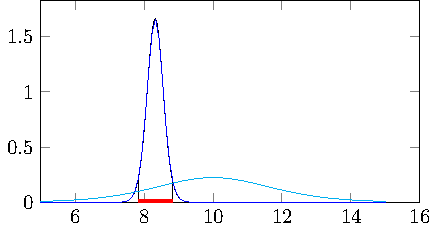
\includegraphics[page = 1]{3º Trabalho/Tikz - pdf/Tikz2.pdf}
        \caption{Caso em que $\frac{\beta_0}{\alpha_0} = \frac{1}{4}$.}
    \end{figure}
    \begin{figure}[H]
        \includegraphics[page = 2]{3º Trabalho/Tikz - pdf/Tikz2.pdf}
        \caption{Caso em que $\frac{\beta_0}{\alpha_0} = \frac{1}{25}$.}
    \end{figure}
    \begin{figure}[H]
        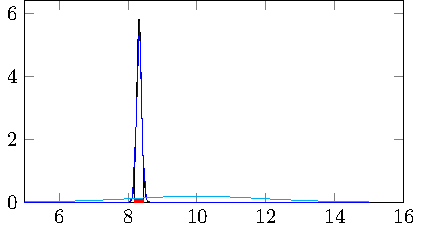
\includegraphics[page = 1]{3º Trabalho/Tikz - pdf/Tikz3.pdf}
        \caption{Caso em que $\frac{\beta_0}{\alpha_0} = \frac{29}{200}$.}
    \end{figure}
    \begin{figure}[H]
        \includegraphics[page = 2]{3º Trabalho/Tikz - pdf/Tikz3.pdf}
        \caption{Caso em que $\frac{\beta_0}{\alpha_0} = \frac{1}{10}$.}
    \end{figure}
\end{multicols}

Dessa forma, podemos ver que o intervalo de credibilidade varia conforme nossa escolha de priori. E, como estamos sob o paradigma bayesiano, podemos interpretar o intervalo de credibilidade de 95\% como um intervalo em que temos 95\% de probabilidade de $\mu$ estar ali. Note que essa interpretação pode ser contraditória pois, como visto acima, esse intervalo varia conforme nossa escolha de priori, entretanto, quando $n$ cresce, o intervalo de credibilidade diminui, ou seja, a variância a posteriori de $\mu$ diminui e, consequentemente, temos mais certeza sobre a distribuição de $\mu$. Para ilustrar isso fiz algumas contas e simulações no Notebook Python que pode ser encontrado no GitHub.

\subsubsection*{Uma outra solução}

De forma análoga a anterior, precisamos apenas encontrar os valores de $\mu_0$, $\alpha_0$, $\beta_0$ e $\mu_0$. Feito isso, podemos fazer o cálculo da posteriori, isto é, a atualização desses parâmetros.

De acordo com o enunciado, Palmirinha acha que $\mu$ tem média $10$ e desvio padrão igual a $2$, ou seja, tomando $\alpha_0 > \frac{1}{2}$, podemos dizer que, pelo Teorema 8.6.3 do DeGroot \cite{degroot}, $E[\mu] = \mu_0$. Dessa forma, podemos definir $\mu_0 = 10$ e, por enquanto, $\alpha_0 > \frac{1}{2}$. Além disso, o mesmo teorema afirma que, se $\alpha_0 > 1$, então
\[Var(\mu) = \dfrac{\beta_0}{\lambda_0 \left(\alpha_0 - 1\right)} \implies \lambda_0 = \dfrac{\beta_0}{Var(\mu) \left(\alpha_0 - 1\right)},\]

\noindent ou seja, escolhendo $Var(\mu) = 4$, conforme suspeita a priori de Palmirinha, temos $\lambda_0$ a partir das escolhas e $\beta_0$ e $\alpha_0$, com este último maior que $1$.

Agora, manipulando o coeficiente de variação, temos que
\begin{equation*}
    \begin{split}
        \operatorname{cv} & = \dfrac{\sigma}{\mu} \\
        & = \dfrac{\sqrt{\sigma^2}}{\mu} \\
        & = \dfrac{\sqrt{\tau^{-1}}}{\mu} \\
        & = \dfrac{1}{\mu \sqrt{\tau}}.
    \end{split}
\end{equation*}

Assim, se temos que o coeficiente de variação é de $\frac{1}{2}$, conforme suspeita da Palmirinha, então vale que
\[\dfrac{1}{2} = \dfrac{1}{\mu \sqrt{\tau}} \implies \tau = \dfrac{4}{\mu^2}.\]

Agora, podemos supor um $\mu$ fixo, dessa forma, temos que
\[E[\tau] = \dfrac{4}{\mu^2}.\]

Escolhendo para fixar $\mu$ podemos pensar em tomar $\mu_0$ como valor para $\mu$, o que é razoável dado que $\mu_0$ é a média e a moda a priori para $\mu$. Dessa forma, temos que
\[\dfrac{\alpha_0}{\beta_0} = \dfrac{4}{\mu_0^2} \implies \dfrac{\alpha_0}{\beta_0} = \dfrac{1}{25}.\]

Como temos que $\alpha_0 > 1$, podemos tomar $\alpha_0 = 2$ e, consequentemente, $\beta_0 = 50$. Dessa forma,
\[\lambda_0 = \dfrac{50}{4 \left(2 - 1\right)} = \dfrac{25}{2}\]

\noindent e, com isso, podemos atualizar os parâmetros. Temos
\begin{equation*}
    \left\{
        \begin{array}{ll}
            \alpha_0 & = 2 \\
            \beta_0 & = 50 \\
            \mu_0 & = 10 \\
            Var(\mu) & = 4 \\
            n & = 10 \\
            \overline{x}_n & = 8.307849 \\
            \overline{s}_n^2 & = 7.930452 \\
            \lambda_0 & = 12.5,
        \end{array}
    \right.
\end{equation*}

\noindent o que nos gera os seguintes parâmetros a posteriori:
\begin{equation*}
    \left\{
        \begin{array}{ll}
            \lambda_1 & = 22.5 \\
            \mu_1 & = 9.247932888888888 \\
            \alpha_1 & = 7 \\
            \beta_1 & = 61.91904546333612
        \end{array}
    \right.
\end{equation*}

\noindent e o intervalo de credibilidade igual a $(7.903138300680498, 10.592727477097279)$.

Note que, na solução acima, precisamos escolher apenas um valor para $\alpha_0$. Assim, podemos nos perguntar o que aconteceria com um $\alpha_0$ diferente. Chutando um pouco o balde e escolhendo $\alpha_0 = 100$, consequentemente $\beta_0 = 2500$, obtemos algumas alterações nos demais parâmetros a posteriori e, no fim, uma pequena modificação no intervalo de credibilidade, o qual passa a ser $(6.576604381280694, 11.348808015004133)$. Graficamente, temos os seguintes cenários:
\begin{multicols}{2}
    \begin{figure}[H]
        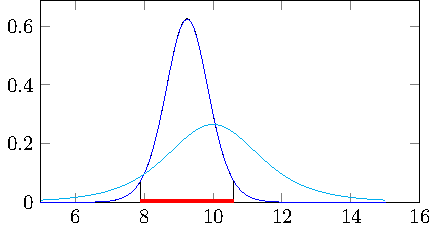
\includegraphics[page = 1]{3º Trabalho/Tikz - pdf/Tikz4.pdf}
        \caption{Distribuição de $\mu$ quando $\alpha_0 = 2$.}
    \end{figure}
    \begin{figure}[H]
        \includegraphics[page = 2]{3º Trabalho/Tikz - pdf/Tikz4.pdf}
        \caption{Distribuição de $\mu$ quando $\alpha_0 = 100$.}
    \end{figure}
\end{multicols}

Note que com $\alpha_0$ maior temos um intervalo de credibilidade maior a posteriori, ou seja, nossa distribuição a posteriori de $\mu$ tem maior variância. Agora, mantendo a média, variância amostral e parâmetros iniciais, mas mudando $n$ para $100$, como se Valciclei tivesse amostrado mais pamonhas. Fazendo isso, temos as seguintes distribuições para $\mu$:
\begin{multicols}{2}
    \begin{figure}[H]
        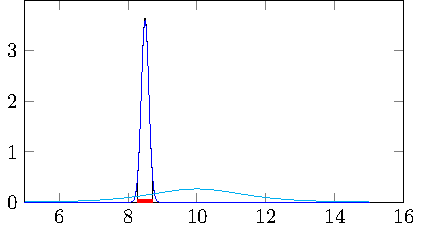
\includegraphics[page = 1]{3º Trabalho/Tikz - pdf/Tikz5.pdf}
        \caption{Distribuição de $\mu$ quando $\alpha_0 = 2$ e $n = 100$.}
    \end{figure}
    \begin{figure}[H]
        \includegraphics[page = 2]{3º Trabalho/Tikz - pdf/Tikz5.pdf}
        \caption{Distribuição de $\mu$ quando $\alpha_0 = 100$ e $n = 100$.}
    \end{figure}
\end{multicols}

Note que, a medida com que $n$ cresce, o intervalo de credibilidade diminui mostrando, assim como dito anteriormente, que a distribuição de $\mu$ fica mais concentrada, com variância menor e, dessa forma, podemos ver as posteriores tendem a convergir para uma mesma distribuição, mesmo com prioris com $\alpha_0$ distintos.

\section*{Conclusão}

Já no início pudemos ter uma boa ideia do significado da precisão, sendo visualizada como uma métrica de proximidade dos dados em relação a média. Após isso passamos a fazer uma análise bayesiana com a normal com média e precisão desconhecidas. Feita a análise, descobrimos mais uma família conjugada, agora com duas distribuições a priori. Além disso, a visualização de $\lambda_0$ como um nível de certeza a priori acabou deixando o cálculo da média a posteriori, $\mu_1$, um pouco mais intuitivo. Além dele, vimos que $\alpha_0$ e $\beta_0$ são hiperparâmetros que irão contribuir na forma da posteriori de $\mu$, ditando a concentração em torno de $\mu_1$.

Chegando no exemplo vimos que a escolha da priori tem certa relevância no cálculo da posteriori, embora os intervalos de credibilidade que foram gerados ficaram próximos. Além disso, vimos que a medida em que $n$ cresce essa relevância  da priori diminui. Ou seja, a priori pode ser gerada de diversas formas, a depender da interpretação de quem vai elaborá-la, mas a posteriori nos dará resultados similares e, com uma grande amostragem, as posterioris tendem a uma mesma distribuição.

Assim, uma das maiores lições desse trabalho é que elicitar prioris pode ser muito complicado, podendo ser considerada uma arte na qual o ponto de vista e interpretação do artista pode ser crucial para obtermos um resultado razoável ou então um totalmente descartável.

Por fim, talvez seria interessante alguém falar com Palmirinha para ela buscar um assistente menos comilão, imagine ele fazendo uma amostragem de $100$ pamonhas!

\printbibliography

\end{document}
